\subsection{Unirse a una partida}

\begin{figure}[ht]
\centering
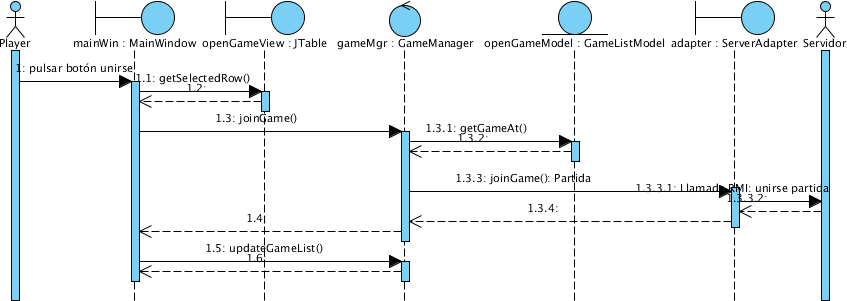
\includegraphics[scale=0.6]{img/ch03devel-joingame.png}
\caption{Diagrama de secuencia de ``Unirse a una partida''}
\end{figure}

Al seleccionar una partida listada en la vista de partidas disponibles, se
activará el botón para unirse a ella. Al pulsar este botón, la ventana
principal obtendrá el índice de la partida seleccionada y llamará a la función
correspondiente del gestor de partidas.

Utilizando el índice proporcionado desde la interfaz, el gestor de partidas
obtendrá el objeto \texttt{GameInfo} que representa a la partida seleccionada.
A continuación pedirá al \texttt{ServerAdapter} que efectúe la unión a la
partida en el servidor.

Al igual que ocurría en el caso de uso anterior, se llamará a la funcionalidad
de actualizar la lista de partidas para que la interfaz muestre los cambios
producidos.
